% CS224W project milestone -- Autumn 2026
% Compile: `tectonic main.tex` (or pdflatex + bibtex). Figures: `python figures/make_figures.py` from the repository root.
% The milestone is credit/no credit: code plus a report draft (problem, data and processing, model design and metrics).
\documentclass{article}

\usepackage[final]{neurips_2022}
\makeatletter
\renewcommand{\@noticestring}{CS224W: Machine Learning with Graphs, Stanford University, Autumn 2026. Project milestone (type 1: real-world application).}
\makeatother

\usepackage{xcolor}
\definecolor{mappath}{HTML}{9E5400}
\definecolor{graphpath}{HTML}{0B6065}
\usepackage[utf8]{inputenc}
\usepackage[T1]{fontenc}
\usepackage[colorlinks=true,linkcolor=black,citecolor=graphpath,urlcolor=graphpath]{hyperref}
\usepackage{url}
\usepackage{booktabs}
\usepackage{amsfonts,amsmath}
\usepackage{microtype}
\usepackage{graphicx}
\usepackage{tikz}
\usetikzlibrary{arrows.meta,positioning,fit}

\title{Where Should a Robot Swarm See Its Neighbors?\\ Communication-Range Transfer in a GNN Coverage Policy}

\author{%
  Lo\"ic Poisson \quad Harold Gardon \quad Claire Fitussi \\
  Stanford University \\
  \texttt{\{lpoisson, gardon21, cfitussi\}@stanford.edu}
}

\begin{document}
\maketitle
\vspace{-1em}

\paragraph{Status in one paragraph.}
Since the proposal we have (i) finished the diagnosis of LPAC's failure when the communication range grows, (ii) implemented and trained six variants of the policy (three seeds each, 25 training runs on a FarmShare L40S GPU), and (iii) found the first trained model whose coverage improves when robots hear farther: a GNN layer that reads \emph{bounded} relative geometry on the edges (V4). We also learned two methodological lessons that change how we will report results. This draft is organized as the final blog post will be: motivation, data, model, results, and what remains.

% =====================================================================
\section{Problem and motivation}
% =====================================================================
In \emph{coverage control}, $N$ robots spread over an area so that their sensors watch the regions that matter, given by an importance density field (IDF) $\phi$ unknown in advance~\citep{cortes2004coverage}. Each robot sees only a $64\times64$\,m footprint and talks only to robots within its \emph{communication range}~$R$. The communication network is the graph $G_R=(V,E_R)$, with an edge $(i,j)$ whenever $\|p_i-p_j\|\le R$, so decentralized control is a graph learning problem: each robot decides what to send to its neighbors and how to combine what it receives~\citep{tolstaya2019flocking}.

LPAC~\citep{agarwal2025lpac} is a recent GNN policy for this task. Its authors report that it degrades when $R$ grows (their Sec.~VI-H, Fig.~20) and hypothesize that aggregating many messages loses information. This matters in practice: a radio's range changes with terrain and hardware, and a fleet may mix robots with different radios. A policy that gets \emph{worse} when robots communicate \emph{more} cannot be deployed safely. Our question is therefore: \emph{where should neighbor geometry enter a GNN policy, and at which scale, so that the policy transfers across communication ranges and benefits from longer ones?}

% =====================================================================
\section{Data, processing and metric}
% =====================================================================
\paragraph{Dataset.} We use the public \textbf{CoverageControl} library~\citep{coveragecontrol} (GPL-3.0, release v1.3.1): a simulator of 32 robots in a $1024\times1024$\,m world whose IDFs are mixtures of 32 random Gaussians, the published LPAC checkpoint, its 11 evaluation environments, and scripts that generate imitation data from a \emph{clairvoyant} centroidal-Voronoi (CVT) controller that knows $\phi$ and every position.

\paragraph{Processing.} One sample is the state of all 32 robots at one time step: four $32\times32$ maps per robot (local importance, two neighbor-map channels, obstacles), the positions, the graph $G_R$ and the clairvoyant velocity as target. As in the paper, a training set has 100{,}000 samples. We generated sets at 128, 256, 512 and 1024\,m, merged them into a \emph{mixed-range} set, and wrote a redrawing tool that rebuilds the neighbor maps of an existing set at any scale (it recovers each sample's range from its stored edge weights), so a new map encoding does not require re-simulating. We also generated 40 new evaluation environments.

\paragraph{Task and metric.} The policy maps local observations and messages to a velocity (node-level regression on $G_R$), trained by imitation with a mean-squared error. We evaluate it in closed loop for 600 steps with the paper's metric: the coverage cost $J=\int\phi(q)\min_i\|q-p_i\|^2\,dq$ averaged over the episode and divided by the clairvoyant's cost on the same environment (lower is better). We vary the \emph{test-time} range $R\in\{128,256,512,768,1024\}$\,m. Baselines are the centralized CVT (about 2.3--2.5) and the published model.

\paragraph{Protocol and noise.} Evaluation is deterministic on Intel CPU nodes (AMD nodes round convolutions differently). Differences between models are paired by environment. We report the 40 new environments as the primary set: two runs of the same recipe differ there by 0.01--0.05, against 0.08--0.15 on the 11 released ones (Sec.~\ref{sec:lessons}).

% =====================================================================
\section{Model design}
% =====================================================================
\begin{figure}[t]
\centering
\resizebox{0.62\linewidth}{!}{%
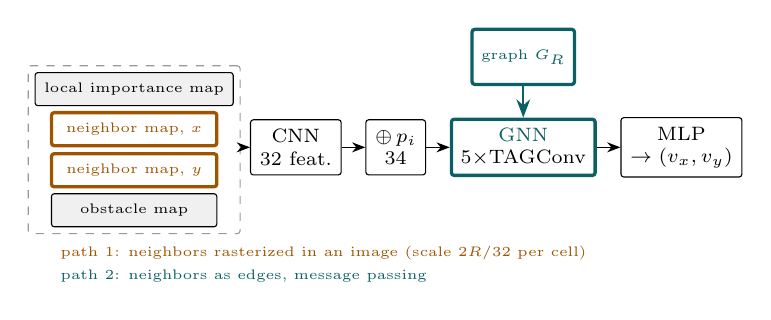
\begin{tikzpicture}[font=\scriptsize, >=Stealth,
  box/.style={draw, rounded corners=1pt, minimum height=7mm, align=center, fill=white},
  inp/.style={draw, rounded corners=1pt, minimum width=21mm, minimum height=4.2mm, align=center, font=\tiny}]
  \node[inp, fill=black!6] (loc) {local importance map};
  \node[inp, draw=mappath, very thick, below=0.6mm of loc] (mx) {\textcolor{mappath}{neighbor map, $x$}};
  \node[inp, draw=mappath, very thick, below=0.6mm of mx] (my) {\textcolor{mappath}{neighbor map, $y$}};
  \node[inp, fill=black!6, below=0.6mm of my] (obs) {obstacle map};
  \node[box, right=4mm of mx.south east, anchor=west] (cnn) {CNN\\32 feat.};
  \node[box, right=3mm of cnn] (cat) {$\oplus\,p_i$\\34};
  \node[box, draw=graphpath, very thick, right=3mm of cat] (gnn) {\textcolor{graphpath}{GNN}\\5$\times$TAGConv};
  \node[box, draw=graphpath, very thick, above=4mm of gnn, font=\tiny] (graph) {\textcolor{graphpath}{graph $G_R$}};
  \node[box, right=3mm of gnn] (mlp) {MLP\\$\to(v_x,v_y)$};
  \node[draw=black!40, dashed, rounded corners=1pt, inner sep=0.8mm, fit=(loc)(obs)] (inputs) {};
  \draw[->] (inputs.east |- cnn.west) -- (cnn.west);
  \draw[->] (cnn) -- (cat); \draw[->] (cat) -- (gnn); \draw[->] (gnn) -- (mlp);
  \draw[->, graphpath, thick] (graph) -- (gnn);
  \node[font=\tiny, text=mappath, align=left, below=1.2mm of obs.south west, anchor=north west] {path 1: neighbors rasterized in an image (scale $2R/32$ per cell)};
  \node[font=\tiny, text=graphpath, align=left, below=4.2mm of obs.south west, anchor=north west] {path 2: neighbors as edges, message passing};
\end{tikzpicture}}
\caption{LPAC on one robot. Neighbors enter twice: drawn in a $32\times32$ neighbor map read by the CNN (path~1), and as edges of $G_R$ read by the GNN (path~2).}
\label{fig:arch}
\end{figure}

\paragraph{LPAC.} Each robot runs the same network (Fig.~\ref{fig:arch}). A CNN encodes the four maps into 32 features, the position is appended, five TAGConv layers~\citep{du2017tagconv} with $K=3$ exchange information over $G_R$, and an MLP outputs the velocity:
\begin{equation}
X^{(\ell+1)}=\mathrm{ReLU}\Big(\textstyle\sum_{k=0}^{K}\big(D^{-1/2}AD^{-1/2}\big)^{k}X^{(\ell)}W_k^{(\ell)}\Big).
\end{equation}
In the \emph{neighbor map}, robot $j$ within range is written into cell $c_{ij}=\mathrm{round}\big((p_j-p_i)\tfrac{32}{2R}+15.5\big)$ with value $(p_j-p_i)/R$. The map therefore zooms out with $R$: a cell is 8\,m wide at 128\,m and 64\,m at 1024\,m, and a model trained at one range sees images at test time that it never saw in training.

\paragraph{Variants.} All variants keep the TAGConv stack and the training recipe (imitation, Adam, best validation checkpoint) and change only how neighbor geometry is encoded. \emph{Mixed} means trained on the merged 128--1024\,m set.
\begin{itemize}\setlength\itemsep{1pt}
\item \textbf{A}: LPAC with the neighbor map drawn at a fixed 256\,m scale (cells of 16\,m, neighbors within $\min(R,256)$\,m).
\item \textbf{V1}: no neighbor map. \textbf{V2}: GATv2~\citep{brody2022gatv2} with $p_j-p_i$ as edge feature instead of TAGConv.
\item \textbf{V3}: V1 plus a residual PointNet layer~\citep{qi2017pointnetpp} before the TAGConv stack, with edge input $(p_j-p_i)/256$\,m.
\item \textbf{V4} (bounded edges): V3 with an edge input that stays in $[-1,1]$ at every range. With $d_{ij}=\|p_j-p_i\|$,
\begin{equation}
e_{ij}=\Big[\tfrac{p_j-p_i}{d_{ij}},\;\tanh\!\big(\tfrac{d_{ij}}{256}\big)\Big],\qquad
h_i = x_i + \mathrm{ReLU}\Big(g\big(\max_{j\in\mathcal N(i)\cup\{i\}} f([x_j, e_{ij}])\big)\Big),
\end{equation}
with $f,g$ two-layer MLPs, max aggregation (invariant to the number of neighbors, about 2 at 128\,m and 30 at 1024\,m) and $e_{ii}=0$ for the self-loop.
\item \textbf{V5} (multi-scale maps): LPAC with three neighbor-map pairs at fixed scales $s\in\{256,512,1024\}$\,m, each holding the neighbors within $\min(R,s)$, so the CNN reads 8 channels.
\item \textbf{V6}: V5 plus the V4 edge layer.
\end{itemize}

% =====================================================================
\section{Results so far}
% =====================================================================
\paragraph{1. The collapse comes from the image, not from the graph.} Retrained, LPAC matches the published model (1.74 vs 1.69 at 256\,m). Trained at 128\,m, it reaches 5.22 at 1024\,m (6.15 on the 40 new environments), worse than the centralized CVT. A factorial intervention at inference separates the two paths. Capping $G_R$ to the 4 nearest neighbors leaves the cost at 5.11. Redrawing only the neighbor map at a fixed 256\,m scale, with the full graph, brings it to 1.71 (paired $+0.02\pm0.16$ against 256\,m). This holds for every model and on the 40 new environments, and the effective rank of TAGConv outputs never collapses, which rules out over-smoothing. The paper's hypothesis, a lossy aggregation of many messages, is therefore not the cause in transfer.

\begin{table}[t]
\centering
\small
\caption{Cost / clairvoyant cost (lower is better), 40 new environments, mean over three training seeds (six runs for V5). The inference-time fix is shown for reference; all other rows are trained models used as is.}
\label{tab:main}
\begin{tabular}{lccccc}
\toprule
Model & 128\,m & 256\,m & 512\,m & 768\,m & 1024\,m \\
\midrule
LPAC published (trained 128\,m) & 1.96 & 1.70 & 2.87 & -- & 6.15 \\
\quad + fixed 256\,m map at inference & -- & 1.70 & 1.71 & -- & 1.77 \\
Centralized CVT & 2.33 & 2.33 & 2.33 & -- & 2.33 \\
\midrule
A: fixed map, mixed & 2.09 & 1.91 & 1.91 & 1.91 & 1.92 \\
V3: PointNet edges, trained 128\,m & 2.13 & 2.03 & 2.25 & 2.39 & 2.44 \\
V4: bounded edges, trained 128\,m & 2.05 & 1.87 & 1.90 & 1.90 & 1.90 \\
\textbf{V4: bounded edges, mixed} & 2.14 & 1.87 & \textbf{1.81} & \textbf{1.81} & \textbf{1.82} \\
V5: multi-scale maps, mixed & 2.09 & 1.89 & 1.89 & 1.90 & 1.90 \\
V6: V5 + V4, mixed & 2.12 & 1.91 & 1.87 & 1.88 & 1.89 \\
\bottomrule
\end{tabular}
\end{table}

\begin{figure}[t]
\centering
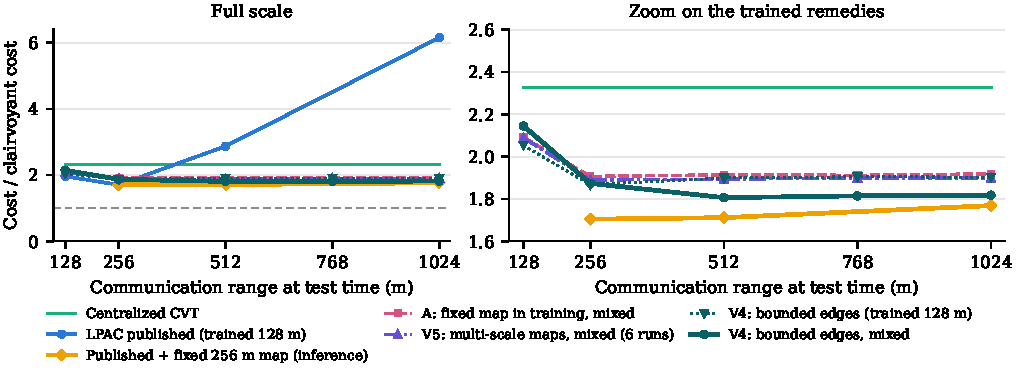
\includegraphics[width=\linewidth]{figures/ranges.pdf}
\caption{Cost against test-time range on the 40 new environments. Left: the published model collapses. Right: every trained remedy removes the collapse; only V4 trained on mixed ranges gets better beyond 256\,m.}
\label{fig:ranges}
\end{figure}

\paragraph{2. Bounded geometry on the edges removes the collapse.} Table~\ref{tab:main} and Fig.~\ref{fig:ranges} compare the trained remedies. Removing the map (V1) costs 0.75 at 256\,m, and GATv2 on raw relative positions (V2) underfits. V3's PointNet layer degrades with range because its inputs grow with $R$. V4 replaces them with a unit direction and a saturating distance: \emph{trained at 128\,m only}, it no longer collapses (1.90 at 1024\,m, three seeds) and beats V3 at every range, beyond seed noise.

\paragraph{3. A first model that benefits from a longer range.} Trained on mixed ranges, V4 is the only model whose cost \emph{decreases} from 256 to 1024\,m: $-0.055$ (SE 0.016, 27/40 environments better) on the new environments and $-0.12$ (SE 0.03, 10/11) on the released ones, in each of the three seeds. A and V5 are flat, which means they tolerate a longer range without using it. V6 behaves exactly like V5 (within 0.03 at every range), so the two encodings do not add up. No trained model yet reaches LPAC's 256\,m level: at 256\,m all stay 0.05--0.09 behind LPAC retrained at that range (1.82 on the new environments).

\begin{figure}[t]
\centering
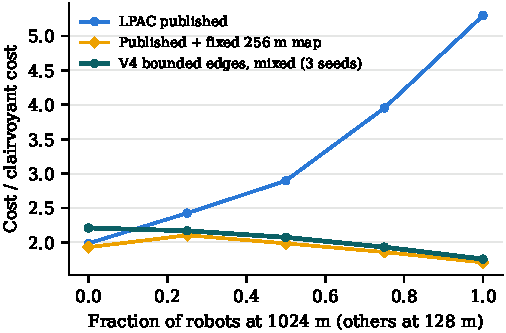
\includegraphics[width=0.55\linewidth]{figures/hetero.pdf}
\caption{Heterogeneous teams on the 11 released environments: a fraction of the robots hears at 1024\,m, the others at 128\,m (8 random draws for LPAC, 4 per seed for V4).}
\label{fig:hetero}
\end{figure}

\paragraph{4. Heterogeneous teams.} When a fraction $f$ of the robots hears at 1024\,m and the rest at 128\,m (Fig.~\ref{fig:hetero}), the published model's cost grows from 1.98 to 5.30. With V4 (mixed), each robot that hears farther helps: the cost falls at every step of $f$ for each seed, by $0.45$ in total (SE 0.08, 11/11 environments). This matches the inference-time fix within noise ($+0.05$ to $+0.09$, SE 0.08) for $f\ge\tfrac14$, without any test-time change. V4 remains 0.28 behind when every robot is at 128\,m, its weakest range.

\paragraph{5. Two methodological lessons.}\label{sec:lessons}
\emph{(a) Run-to-run noise.} Training is not bit-reproducible at a fixed seed (GPU scatter operations, parallel data loading). Two launches of V5 with the same seed differ by 0.08--0.15 at 256\,m on the 11 released environments, more than the spread between seeds of one launch. A first set of three V5 runs appeared to match LPAC at 256\,m (1.78); pooled with three more, it is 0.10 behind. We now report the 40 new environments as primary and will use six or more runs per recipe for any claim at the 0.05 level. \emph{(b) Validation loss does not predict coverage.} Map-based models reach their best validation MSE at epoch 4--6, after which it rises from 0.46 to 0.54 while the coverage cost does not move: epoch-25 checkpoints of V5 and V6 match their best-validation checkpoints within 0.04. Imitation loss is therefore a poor model-selection signal for this task.

% =====================================================================
\section{Code}
% =====================================================================
The repository\footnote{\url{https://github.com/loicpoisson/lpac-communication-range} (private until the final submission; access on request).} contains: \texttt{lpac\_study/}, a Python package around CoverageControl and PyTorch Geometric~\citep{fey2019pyg} with the closed-loop evaluation (\texttt{episode.py}, \texttt{sweep.py}), the inference-time interventions on the graph and the map (\texttt{factorial.py}, \texttt{neighbourhood.py}), the variants V0--V6 (\texttt{variants.py}), heterogeneous teams (\texttt{heterogeneous.py}), the specialist mixture (\texttt{mixture.py}) and the analyses (effective rank, CKA, checkpoint selection); \texttt{training/}, data generation, map redrawing and the Slurm launchers for FarmShare; \texttt{tests/}, unit tests of the variants (bounds and scale behavior of the V4 features, equality of V5's 256\,m pair with the fixed map, V6 reducing to V5 when its edge layer is zeroed); the result tables and a running journal of every experiment. An early notebook (\texttt{lpac\_eval.ipynb}) runs the evaluation of the published model; it will grow into the Colab.

% =====================================================================
\section{Plan to the final submission}
% =====================================================================
\begin{enumerate}\setlength\itemsep{1pt}
\item \textbf{Firm up the main claims}: six runs for LPAC retrained at 256\,m, A, V4 mixed and V5 mixed, so that the 256\,m gap and the range gain are measured against run-to-run noise.
\item \textbf{Close V4's gap at short range}: V4 is weak at 128\,m (2.14). We will try weighting the mixed set toward short ranges and a learned scale in the saturating distance.
\item \textbf{Information loss vs.\ distribution shift}: draw the same neighbors in a finer map to test whether the 256\,m map discards useful information.
\item \textbf{Deliverables}: the Colab (data loading, model definitions in PyG, training on a reduced set, closed-loop evaluation of the released checkpoints) and the Medium post built on Figs.~\ref{fig:arch}--\ref{fig:hetero}.
\end{enumerate}

\bibliographystyle{plainnat}
\small
\bibliography{refs}

\end{document}
